%%%% ijcai11.tex

\typeout{IJCAI-13 Instructions for Authors}

% These are the instructions for authors for IJCAI-13.
% They are the same as the ones for IJCAI-11 with superficical wording
%   changes only.

\documentclass{article}
% The file ijcai13.sty is the style file for IJCAI-13 (same as ijcai07.sty).
\usepackage{ijcai13}
\usepackage{graphicx}
\usepackage{algorithmic}
\usepackage{algorithm}

% Use the postscript times font!
\usepackage{times}

% the following package is optional:
%\usepackage{latexsym} 

% Following comment is from ijcai97-submit.tex:
% The preparation of these files was supported by Schlumberger Palo Alto
% Research, AT\&T Bell Laboratories, and Morgan Kaufmann Publishers.
% Shirley Jowell, of Morgan Kaufmann Publishers, and Peter F.
% Patel-Schneider, of AT\&T Bell Laboratories collaborated on their
% preparation.

% These instructions can be modified and used in other conferences as long
% as credit to the authors and supporting agencies is retained, this notice
% is not changed, and further modification or reuse is not restricted.
% Neither Shirley Jowell nor Peter F. Patel-Schneider can be listed as
% contacts for providing assistance without their prior permission.

% To use for other conferences, change references to files and the
% conference appropriate and use other authors, contacts, publishers, and
% organizations.
% Also change the deadline and address for returning papers and the length and
% page charge instructions.
% Put where the files are available in the appropriate places.

\title{Rapport de projet}
\author{Théo Q, Corto C, Brandon FL \\
Université de Nice\\
France}

\begin{document}

\maketitle


\section{Introduction}



\subsection{Gnuplot}
\begin{figure}[h]
\centering
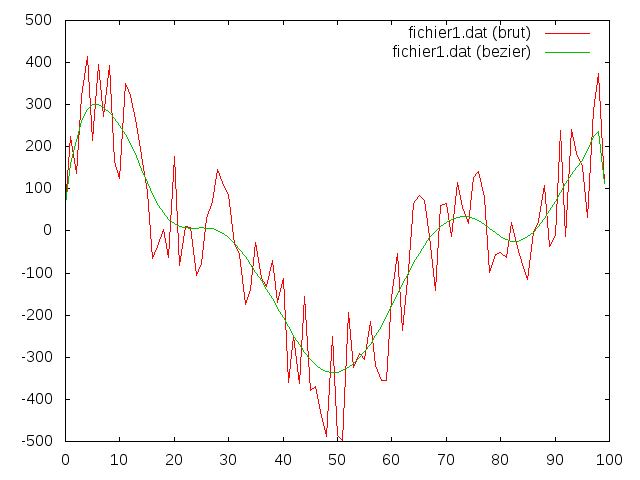
\includegraphics[width=\linewidth]{courbe-fichier1-bezier.png} 
\caption{Titre}
\label{fig:toto}
\end{figure}
voir img\ref{fig:toto}

\subsection{Tableau}
\begin{table}[h]
\centering
\begin{tabular}{|c|c|}
\hline 
130 & 122.3119006607484 \\ 
\hline 
131 & 121.33308199009045 \\ 
\hline 
132 & 122.19824652561799 \\ 
\hline 
133 & 120.6598898351286 \\ 
\hline 
134 & 121.33205925538913 \\ 
\hline 
\end{tabular} 
\caption{Titre}
\label{tab:toto2}
\end{table}


\section{Formule et Algorithme}
\begin{algorithm}[H]
\caption{mon algo ...}
\begin{algorithmic}[1]
\STATE $s =0$
\FOR {$i=1$ to $n$}
\IF {$n \geq 100$}
\STATE $s= s + 1$
\ENDIF
\ENDFOR
\end{algorithmic}
\end{algorithm}

\begin{equation}
f(x)=1 - x^2
\end{equation}
\begin{equation}
g(x)=\frac{sin(x^2)}{x^3}
\end{equation}
\begin{equation}
\zeta(s)= \sum_{n=1}^{+\infty}\frac1{n^s}
\end{equation}

\subsection{Conclusion}
TEXTE

\end{document}

